%%%%%%%%%%%%%%%%%%%%%%%%%%%%%%%%%%%%%%%%%
% Beamer Presentation
% LaTeX Template
% Version 1.0 (10/11/12)
%
% This template has been downloaded from:
% http://www.LaTeXTemplates.com
%
% License:
% CC BY-NC-SA 3.0 (http://creativecommons.org/licenses/by-nc-sa/3.0/)
%
%%%%%%%%%%%%%%%%%%%%%%%%%%%%%%%%%%%%%%%%%

%----------------------------------------------------------------------------------------
%	PACKAGES AND THEMES
%----------------------------------------------------------------------------------------

\documentclass{beamer}

\mode<presentation> {

% The Beamer class comes with a number of default slide themes
% which change the colors and layouts of slides. Below this is a list
% of all the themes, uncomment each in turn to see what they look like.

%\usetheme{default}
%\usetheme{AnnArbor}
%\usetheme{Antibes}
%\usetheme{Bergen}
%\usetheme{Berkeley}
%\usetheme{Berlin}
%\usetheme{Boadilla}
%\usetheme{CambridgeUS}
%\usetheme{Copenhagen}
%\usetheme{Darmstadt}
%\usetheme{Dresden}
%\usetheme{Frankfurt}
%\usetheme{Goettingen}
%\usetheme{Hannover}
%\usetheme{Ilmenau}
%\usetheme{JuanLesPins}
%\usetheme{Luebeck}
\usetheme{Madrid}
%\usetheme{Malmoe}
%\usetheme{Marburg}
%\usetheme{Montpellier}
%\usetheme{PaloAlto}
%\usetheme{Pittsburgh}
%\usetheme{Rochester}
%\usetheme{Singapore}
%\usetheme{Szeged}
%\usetheme{Warsaw}

% As well as themes, the Beamer class has a number of color themes
% for any slide theme. Uncomment each of these in turn to see how it
% changes the colors of your current slide theme.

%\usecolortheme{albatross}
%\usecolortheme{beaver}
%\usecolortheme{beetle}
%\usecolortheme{crane}
%\usecolortheme{dolphin}
%\usecolortheme{dove}
%\usecolortheme{fly}
%\usecolortheme{lily}
%\usecolortheme{orchid}
%\usecolortheme{rose}
%\usecolortheme{seagull}
%\usecolortheme{seahorse}
%\usecolortheme{whale}
%\usecolortheme{wolverine}

%\setbeamertemplate{footline} % To remove the footer line in all slides uncomment this line
%\setbeamertemplate{footline}[page number] % To replace the footer line in all slides with a simple slide count uncomment this line

%\setbeamertemplate{navigation symbols}{} % To remove the navigation symbols from the bottom of all slides uncomment this line
}

\usepackage{graphicx} % Allows including images
\usepackage{booktabs} % Allows the use of \toprule, \midrule and \bottomrule in tables

\usepackage{siunitx} % Provides the \SI{}{} and \si{} command for typesetting SI units
\usepackage{natbib} % Required to change bibliography style to APA
\usepackage{amsmath} % Required for some math elements
\usepackage{verbatim} % Required to comment out large sections

\usepackage{float}
\usepackage{subcaption} 

%----------------------------------------------------------------------------------------
%	TITLE PAGE
%----------------------------------------------------------------------------------------

\title[Documentation on LOA]{Documentation on Lion Optimization Algorithm (LOA) by Maziar Yazdani and Fariborz Jolai} % The short title appears at the bottom of every slide, the full title is only on the title page
\author[Tyrel Dogup, Deo Fetalvero]
{%
   \texorpdfstring{
        \begin{columns}
            \column{.45\linewidth}
            \centering
            Tyrel Justin A. Dogup\\
            \href{mailto:tadogup1@up.edu.ph}{tadogup1@up.edu.ph}
            \column{.45\linewidth}
            \centering
            Deo Franc M. Fetalvero\\
            \href{mailto:dmfetalvero@up.edu.ph}{dmfetalvero@up.edu.ph}
        \end{columns}
   }
   {John Doe \& Jane Doe}
}
\date{\today} % Date, can be changed to a custom date

\begin{document}

\begin{frame}
\titlepage % Print the title page as the first slide
\end{frame}

\begin{frame}
\frametitle{Overview} % Table of contents slide, comment this block out to remove it
\tableofcontents % Throughout your presentation, if you choose to use \section{} and \subsection{} commands, these will automatically be printed on this slide as an overview of your presentation
\end{frame}

%----------------------------------------------------------------------------------------
%	PRESENTATION SLIDES
%----------------------------------------------------------------------------------------

%------------------------------------------------
\section{Introduction} % Sections can be created in order to organize your presentation into discrete blocks, all sections and subsections are automatically printed in the table of contents as an overview of the talk
%------------------------------------------------

\subsection{Overview} % A subsection can be created just before a set of slides with a common theme to further break down your presentation into chunks

\begin{frame}
\frametitle{Overview}
Solving complex optimization problems has been a hot topic the past decade and has garnered large followings most of which are practitioners and researchers. This attention has brought upon the development of new metaheuristic algorithms, many of which are inspired by various phenomena demonstrated by nature.
The paper proposes a new population based algorithm, the Lion Optimization Algorithm (LOA). The distinct lifestyle of lions and their characteristics of utilizing cooperation was made as the motivational basis for the development of this optimization algorithm. The algorithm is also tested against benchmark problems sourced from literature and whose primary solutions was compared with the results of the test. The results also confirm the performance of this algorithm alongside other algorithms used in the paper.
\end{frame}

%------------------------------------------------
\subsection{Optimization}

\begin{frame}
\frametitle{Optimization}
Basically, optimization is searching for the best solutions out of all possible solutions. A best solution can be defined regarding either the most of some measure of success (e.g. revenue) or the least of another measure (e.g. cost). We can be looking at a group of answers or one answer from a set. In solving optimization problems, one's goal is to minimize or maximize a result variable of a function by trying out different parameters for input.
\end{frame}

\begin{frame}
\frametitle{Optimization Algorithms}
Optimization algorithms can be divided into two major categories, as exact and approximate. Exact algorithms guarantee that the optimal solution to the problem will be found in a finite amount of time. There are, however, harder optimization problems that requires the searching of very large solution sets and thus making it impractical to use exact algorithms. As such, the usage of approximate algorithms are necessitated. These algorithms do not guarantee that the optimal solution will be found, but it can find an approximate (sometimes exact) solution to the problem in a relatively short amount of time, sometimes using a less computationally intensive method. Approximate algorithms can be further divided into two major categories as heuristic and metaheuristic algorithms.
\end{frame}

\begin{frame}{Metaheuristic Algorithms}
Metaheuristic algorithms require minimal or no assumptions about the problem being solved. They can be tailored to optimize a specific problem which makes them applicable to a wide variety of problems. A metaheuristic algorithm optimizes a problem by iteratively improving a single or multiple candidate solutions until a desired quality is achieved. LOA is an example of this type of algorithm.
\end{frame}

\subsection{Applications}
\begin{frame}{Applications}
Researchers have made good use of optimization problems such as scheduling problems, data clustering, image and video processing, tuning of neural networks, and pattern recognition.
\end{frame}
\begin{frame}{Application: Scheduling Problems}
Scheduling problems are problems where different difficulty on jobs would take different amount of time that will be processed by different nodes. The problem is to minimize the time that all the nodes would simultaneously get to be finished. Optimization helps find the best job to node assignment to minimize the mean time.
\end{frame}
\begin{frame}{Application: Data Clustering}
Data clustering or cluster analysis is the way to group a set of objects such that objects with the most similarity a group together in clusters. The objects may have one or more properties to identify and the groups may have smaller subgroups that one can also classify. Optimization helps identify the best clustering of an object based on its parameters.

\end{frame}
\begin{frame}{Application: Image and Video Processing}
Image and video processing is the process of adding metadata to an image or video based to what its visual content actually is. An image or video in a computer is represented as pixels or boxes of colors that is displayed on the screen of the viewer. These pixels individually cannot determine the actual content, which is significant to the viewer, of the image and video. Optimization algorithms help computers identify what pixels in an image or video actually represents to the viewer. Such algorithms help with edge detection, segmentation, representation and description of the parts of an image or video.
\end{frame}
\begin{frame}{Application: Tuning of neural networks}
Neural networks can be tuned by its parameters. These parameters talked about are parameters that are constant throughout the run of the network. This parameters may be tuned to get the best performance out of neural network which may also drive the network to learn faster, slower or not at all. Optimization helps to find the best parameters that will drive the system's performance.

\end{frame}

%------------------------------------------------
\section{The Algorithm}
%------------------------------------------------

\begin{frame}{Inspiration for the algorithm}
Lions have displayed cooperation and antagonism especially in hunting. Lions are also socially inclined meaning that they also organize information that other lions have collected and use them for their benefit.
Male lions have radically different social behavior and appearance than the female lions and v.v.
The lions can also be classified if they're residents or nomads. Resident lions create groups called prides, establish their territories and flourish there while nomads take what they need in an area then finds another area to pillage not establishing territories.
\end{frame}
\begin{frame}{Inspiration for the algorithm}
A pride typically would include five females have cubs of both sexes and one or more adult male lions.
As young males would grow they would separate from their birth pride and establish their own prides.
Nomads, who doesn't establish territories, would move about sporadically (whenever they want) and either in pairs or singularly.
Lions usually hunt together in prides. Female lions would work together to surround and swiftly catch the prey. There could also be a hunter female lion who would go out of territory to hunt on their own while the other members of the pride would wait for the lioness to return. But still, coordinated group hunting would bring greater success in prey hunts.
Lions do go mate anytime around the year and females can have more than one reproductive cycle each year. A lioness can also mate with more than one lion when in heat.
Additionally, to mark their territory the pride would place urine all over the place to drive away others who would intrude.
\end{frame}

%------------------------------------------------

\begin{frame}{Idea for the algorithm}
The initially proposed algorithm started an initial population formed by a set of solutions randomly generated labelled as Lions.A percentage $\%N$ of the initial population of solutions are selected as `Nomad Lions' while the rest are the `Resident Lions'. While the nomad lions are individually grouped, the resident lions are then further divided into partitions called `Prides' where a percentage $\%S$ is percentage of the females in the group but in nomad lions, this percentage is reversed, where $\%S$ will be used to identify the males in the nomad lions. The prides are used for the intensification of searching, while the nomads are used for the diversification.
\end{frame}
\begin{frame}{Idea for the algorithm}
Each lion will have a variable pertaining to the best obtained solution for every passing iteration that will be called best visited position and will be updated regularly for every iteration. In each pride, a few random females will be selected to go hunting. These females will encircle the prey and catch it. The males in the pride will roam the territory. The females may mate with one or more resident males then a young male is created. These males may establish their own prides and territory later or may become a nomad.
The nomad lions roams around the search space to find better (places) solutions. A nomad lion may invade and replace a resident male in a pride, driving out that resident male (replacement). Also, a female lion may also migrate to another pride or become a nomad herself. Weak lions, who have not found better prey (solutions) where there is no competition, will die or be killed (stagnation). The process will go on until the stopping condition is satisfied.
\end{frame}

%------------------------------------------------

%------------------------------------------------


\begin{frame}{Proposed Algorithm: Hunting}
In a pride, females would look for a prey to provide food for the pride. The females would fill specific roles to execute certain strategies to encircle the prey and catch it. In general, lions would approximately follow a pattern in hunting. Stander divided lions into seven different stalking roles which would be grouped into by the Left Wings, Centers and Right Wings.
Left Wings and Right Wings both attack the prey from opposite directions in which the idea of Opposition Based Learning is utilized which also is proven to effectively solve optimization problems.
The group with members of the highest finesses (highest revenue, lowest cost) is considered as the Centers while the other two groups are considered as Left and Right Wings.
In the algorithm, the hunters are divided into three groups: Left, Right and Center. The group with highest cumulative finesses is considered to be the Center and the other groups would be Left and Right Wings.
\end{frame}
\begin{frame}{Proposed Algorithm:Hunting}
\begin{figure}[h]
\begin{center}
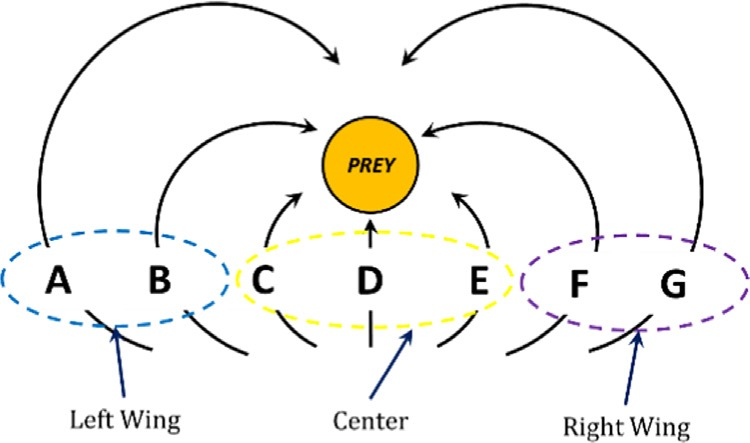
\includegraphics[width=0.65\textwidth]{img/pa/hunting_scheme}
\caption{Generalized lion hunting behavior}
\end{center}
\end{figure}
\end{frame}
\begin{frame}{Proposed Algorithm:Hunting}
A dummy prey would move to a new position and escape as follows:
$$\text{PREY}' = \text{PREY} + \text{rand}(0,1) \times \text{PI} \times (\text{PREY} - \text{Hunter})$$
where PREY is the current position of the prey, PREY$'$ is the new position and PI is the percentage of improvement of the finesse of the hunter.
For the left and right wings, they approach the prey as follows:
\small
\[ \text{Hunter}' =  \begin{cases} 
      \text{rand}((2 \times \text{PREY} - \text{Hunter}), \text{PREY}) & (2 \times \text{PREY} - \text{Hunter}) < \text{PREY} \\
      \text{rand}(\text{PREY}, (2 \times \text{PREY} - \text{Hunter})) & (2 \times \text{PREY} - \text{Hunter}) > \text{PREY}
   \end{cases}
\]
\normalsize
where Hunter is the current position of the hunter and Hunter' is the new position of the hunter.
As for the Center hunters, their new position is as follows:

\[ \text{Hunter}' =  \begin{cases} 
      \text{rand}(\text{Hunter}, \text{PREY}) & \text{Hunter} < \text{PREY} \\
      \text{rand}(\text{PREY}, \text{Hunter}) & \text{Hunter} > \text{PREY}
   \end{cases}
\]
\end{frame}
\begin{frame}{Proposed Algorithm:Hunting}
In all of these equations, $\text{rand}(a,b)$ generates a random number between $a$ and $b$, where $a$ and $b$ are upper and lower bounds, respectively.
In the algorithm, this prey would be a dummy prey put at the start of the phase where PREY would be the midpoint between all the Hunter positions. Each of the hunters would be iterated to attack the dummy prey and the prey would escape to the direction opposite to the new position of the attacking Hunter from the Prey's current position.
\end{frame}
\begin{frame}{Proposed Algorithm:Hunting}
\begin{figure}[h]
\begin{center}
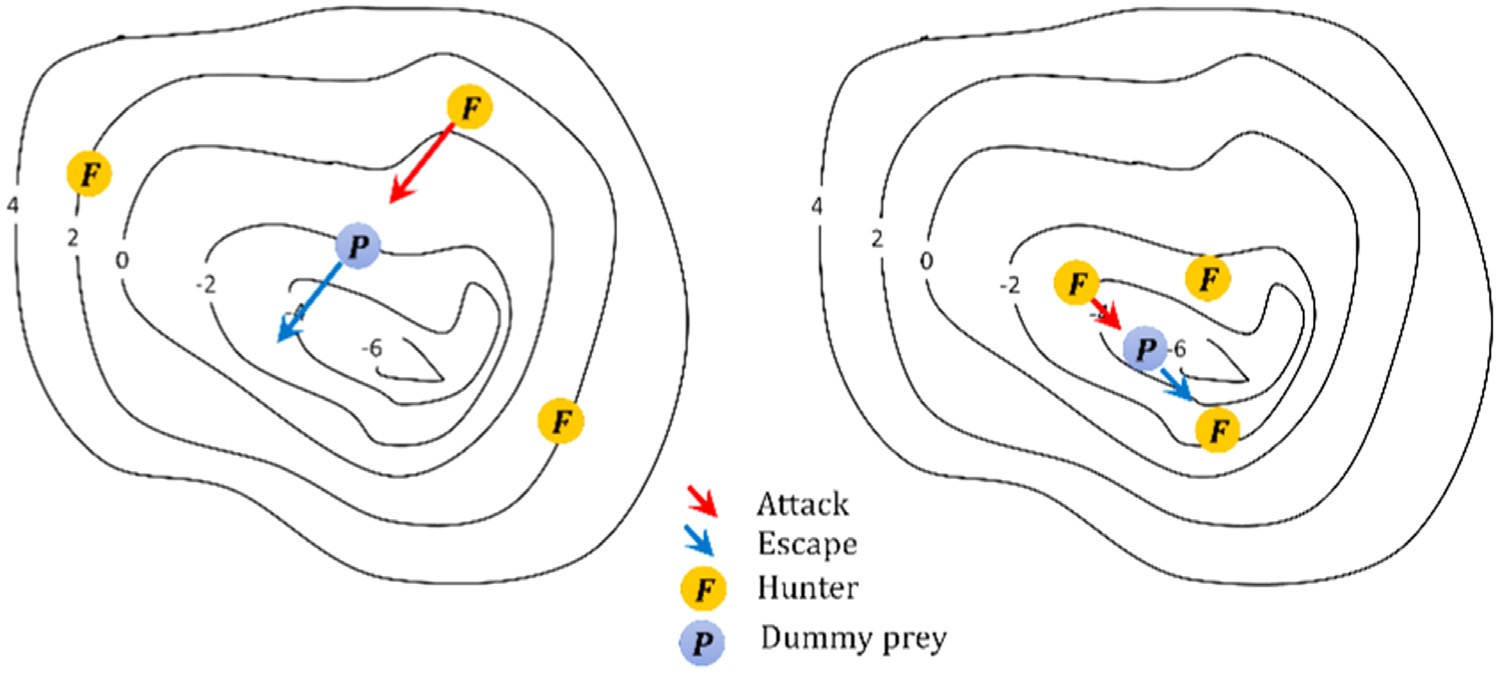
\includegraphics[width=0.65\textwidth]{img/pa/hunting_attack}
\caption{Attack and Escape Example}
\end{center}
\end{figure}
\end{frame}
\begin{frame}{Proposed Algorithm:Hunting}
This mechanism allows the hunters to create a circle shaped neighborhood around the prey, approach it from different directions and catch it. This also allows better solutions to be found (escape local optima) because some hunters use opposite positions.
Therefore hunting in each pride can be stated in the following Pseudo-code:
\begin{figure}[h]
\begin{center}
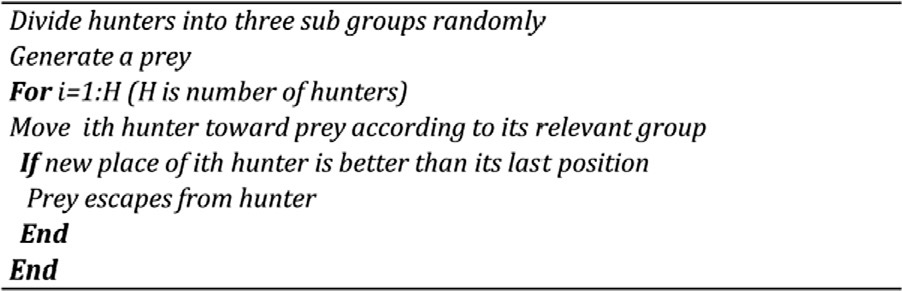
\includegraphics[width=0.65\textwidth]{img/pa/hunting_pseudo}
\end{center}
\end{figure}
\end{frame}

\begin{frame}{Proposed Algorithm: Moving towards safe place}

As mentioned earlier, some of the females go hunting, not all. So, remaining females go toward one of the areas of the territory. In the algorithm, the territories of each pride would consist of personal best solutions so far, which would assist the algorithm to save the best solutions obtained so far over the course of iteration.
Therefore the new position for a female lion is given as:
\begin{align*}
\small
\text{Female Lion}' &= \text{Female Lion} + 2D \times rand(0,1){R1} + U(-1,1) \times \tan(\theta) \times D \\ 
\times {R2} &\text{  where } R1 \cdot R2 = 0, ||R2|| = 1
\normalsize
\end{align*}
where Female Lion and Female Lion' is the previous and next position of the female lion, respectively, and D is the distance between the female lion's position and the selected point chosen by tournament selection in the pride's territory.
{R1} is a vector which its start point is the previous location of the female lion and its direction is toward the selected position. {R2} is perpendicular to {R1}. $\theta$ is an angle that is selected by uniform distribution among $-\pi/6$ and $\pi/6$ and $U$ is a function selecting a random number with uniform distribution.
\end{frame}

\begin{frame}{Proposed Algorithm: Roaming}
Roaming in territory is something lions in a pride usually do. This also helps in getting used to the territory for the lions. For nomads, this is done to find better places to get resources from. In optimization, this can be used to further optimize the local search space for each pride and is used by nomads for searching solutions.

Along with roaming, if a resident male visits a new position better than its current position, update its current best position and best visited solution.

For pride lions, roaming would mean to use each others' position to find better positions (solutions). Similar to the previous section, in this part of the algorithm, the lions would go towards each other using the same formula. 
\end{frame}
\begin{frame}{Proposed Algorithm: Roaming}
For nomad lions, however, roaming would be utilizing random movement to find better positions (solutions). In the algorithm, nomad lions have an advantage to not get stuck in local optima. A nomad lion would randomly roam around the search if space especially when its fitness among the nomads is worse. These nomad lions are only required to check their standing among peer nomads unlike resident lions whom tries to optimize with each others position, thus, giving the nomad lions an advantage to not get stuck. 
\end{frame}
\begin{frame}{Proposed Algorithm: Roaming}
The new position of these nomads are generated using the following equation:

\begin{align*}
 \text{Lion'}_{ij} =
  \begin{cases}
   \text{Lion}_{ij}        & \text{if rand}(0,1)  > pr_i \\
   \text{RAND}_j        & \text{otherwise}
 \end{cases}
\end{align*}

where Lion$_{i}$ is the position of the lion, j is the dimension, rand is a uniformally distributed random number between 0 and 1 and RAND$_j$ is a random position in the search space. Now, $pr_i$ ($i$ for every nomad lion) is represented by:

$$
pr_i = 0.1 + \text{min}\left(0.5, \frac{ (\text{Nomad}_i - \text{Best}_{nomad}) }{ \text{Best}_{nomad} }\right)
$$
\end{frame}
%------------------------------------------------

\begin{frame}{Proposed Algorithm: Mating}
Mating of the lions in the population refers to the mixing of their genes to allow exchanging of information. In this algorithm, for every pride, $\%Ma$ of the females mate with one or more males. For the nomads, $\%Ma$ of the females mate with only one male. These individuals are selected randomly. After mating, two offsprings are produced using the equations:

\small
$$\text{Offspring}_j\text{1}=\beta \times \text{Female Lion}_j +\sum\frac{1-\beta}{\sum_{i=1}^{NR}S_i}\times\text{MaleLion}_j^i\times S_i,$$

$$\text{Offspring}_j\text{2}=(1-\beta) \times \text{Female Lion}_j +\sum\frac{\beta}{\sum_{i=1}^{NR}S_i}\times\text{MaleLion}_j^i\times S_i$$,

\normalsize
where $j$ is dimension; $S_i$ is 1 if male $i$ is selected for mating, 0 otherwise; $NR$ is the number of resident males in a pride; $\beta$ is a randomly generated number with a normal distribution with mean value 0.5 and standard deviation 0.1.
\end{frame}

\begin{frame}{Proposed Algorithm: Mating}
One of these offsprings is set as male, and the other as female. A mutation is applied on each gene of one of the produced offspring with probability $Mu$. Through mutation, a random number replaces the value of the gene.

The purpose of $\beta$ in the equation is to find a value somewhere in between the values of the female and male genes; and the purpose of mutation is to further diversify the solution generated.
\end{frame}

\begin{frame}{Proposed Algorithm: Defense}
When they mature, male cubs in a pride fight with the existing males. The weaker males are driven out of the pride and become nomads. This is done in the algorithm by sorting all the males in the pride according to their fitness. The number of males to be driven out is determined by the sex rate of the pride.

Similarly, nomad males can fight existing males in a pride, and if they prove to be stronger than the resident male, they replace the beaten male in the pride. For each nomad male in the population, it will attack a single or multiple prides determined randomly. Once a pride is selected, the fitness of the nomad male is compared to each resident male of the pride. If the nomad is determined to be stronger, it will replace the resident male, and the resident male becomes a nomad. This behaviour allows the retention of strong lions/solutions in the pride.
\end{frame}

\begin{frame}{Proposed Algorithm: Defense}
\begin{figure}[H]
\begin{center}
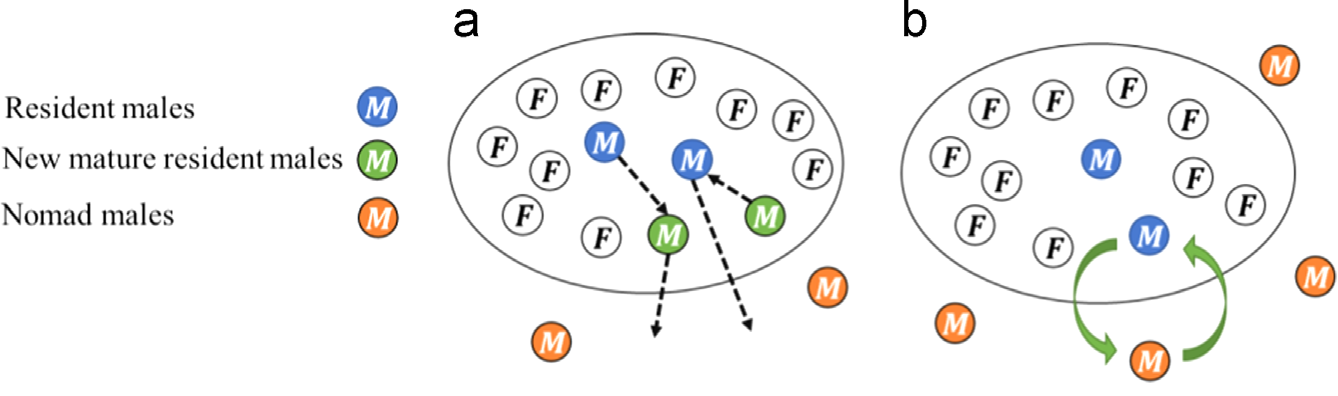
\includegraphics[width=0.7\textwidth]{img/defense/defense}
\caption{(a) Defense against newly matured cubs and (b) Defense against nomads}
\end{center}
\end{figure}
\end{frame}


\begin{frame}{Proposed Algorithm: Migration}
Some females in a pride migrate to another pride or become nomads. Through migration, nomad females can also become residents of a pride. This enhances the diversity of the pride by the best position attained by the migrating females. For each pride, the maximum number of females is determined by the sex rate of the pride. The surplus females plus $\%I$ of the maximum number of females in a pride migrate and become nomads. The nomad females are then sorted according to their fitness and the stronger ones are distributed to random prides to fill the empty place of the migrated females. The number of females to be distributed is determined by the amount of empty female slots of all prides. This procedure allows information sharing among the different prides.
\end{frame}

\begin{frame}{Proposed Algorithm: Equilibrium}
\small
At the end of each iteration of LOA, the number of nomad lions will be controlled with respect to the permitted number of each gender determined by the sex rate. The ones with the least fitness value will be removed from the population. This is to maintain equilibrium in the lion's population.
\normalsize
\begin{figure}[H]
\begin{center}
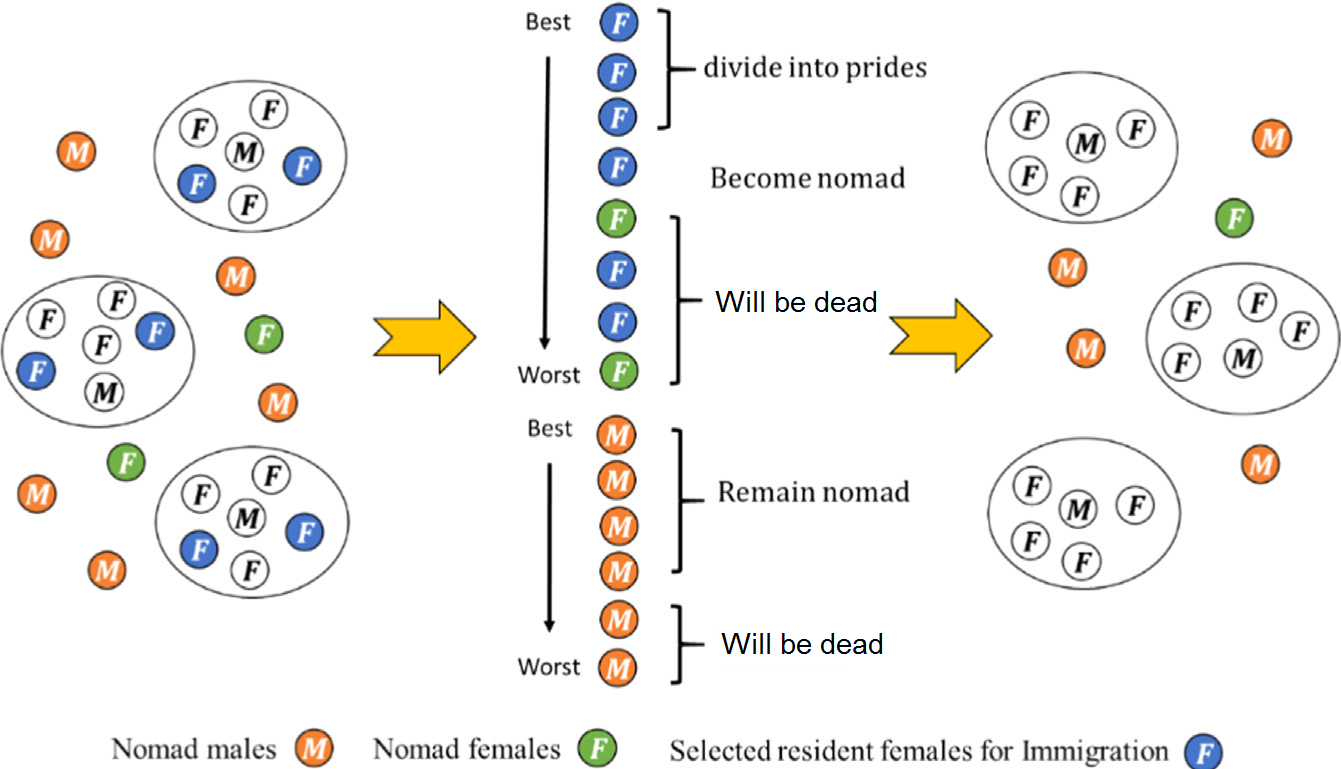
\includegraphics[width=0.6\textwidth]{img/equilibrium/equilibrium}
\caption{Migration and Population Equilibrium}
\end{center}
\end{figure}
\end{frame}


\begin{frame}{The Algorithm}
\begin{figure}[H]
\begin{center}
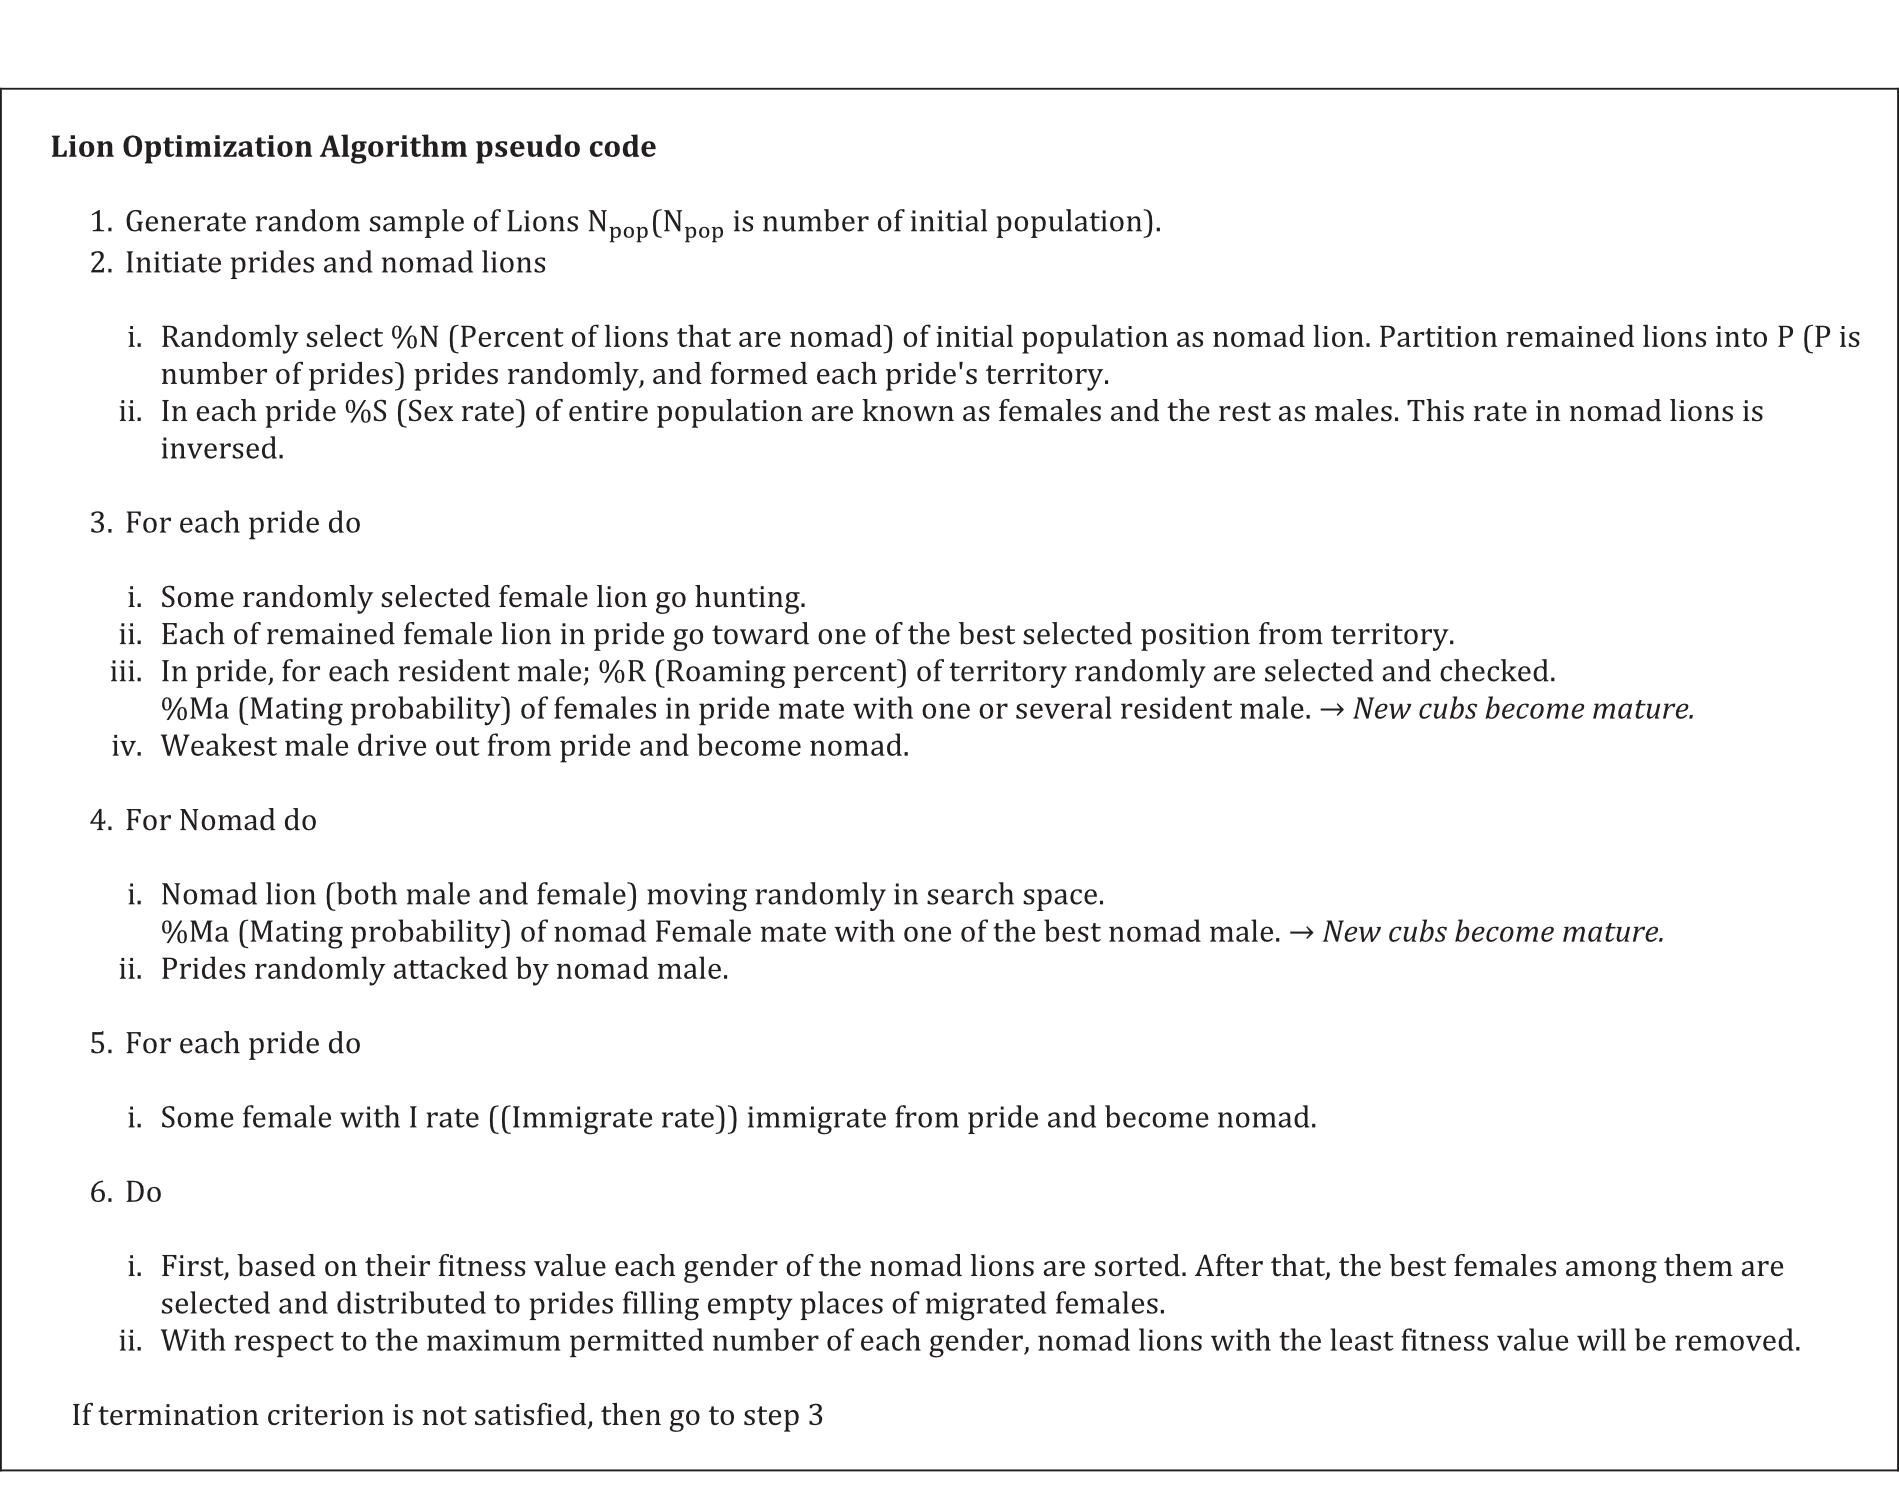
\includegraphics[width=0.8\textwidth]{img/pseudocode}
\caption{The psedocode of LOA}
\end{center}
\end{figure}
\end{frame}

\begin{frame}{Sample Runs }
The algorithm is now tested upon different benchmarking functions. All benchmarks ran using the following parameters of the algorithm.\\
iterations = 300;\\

population = 100;\\

dimension = 2;\\

prides length = 5;\\

percent nomad = 0.2;\\
percent roam = 0.5;\\
percent sex = 0.8;\\

mating rate = 0.3;\\
mutation prob = 0.1;\\

immigration rate = 0.4;\\
\end{frame}

\begin{frame}{Results}
After 300 iterations, the global fitness achieved using each function is graphed against the algorithm's run time. This is displayed in figure 32. The best and worst fitness achieved, along with the standard deviation and median, of each function after 10 runs is also presented in table 3.

\begin{table}[h!]
\centering
\begin{tabular}{l c l c l c l c l}
\hline
 Function & Worst Fitness       & Best Fitness        & Standard Deviation          & Median        \\
\hline
1   & 0.00 & 0.00 & 0.00 & 0.00 \\
\hline
2   & 0.00 & 0.00 & 0.00 & 0.00 \\
\hline
3  & 0.00 & 0.00 & 0.00 & 0.00 \\
\hline
4  & 0.00 & 0.00 & 0.00 & 0.00 \\
\hline
5  & 8.78E-4 & 3.19E-11 & 6.75E-4 & 2.77E-6 \\
\hline
6  & 6.83E-4 & 4.72E-9 & 5.42E-4 & 1.09E-4 \\
\hline
\end{tabular}
\caption{Fitness Results of Functions After 10 Runs}
\end{table}
\end{frame}

\begin{frame}{Results}
\begin{figure}
  \begin{subfigure}[b]{0.4\textwidth}
    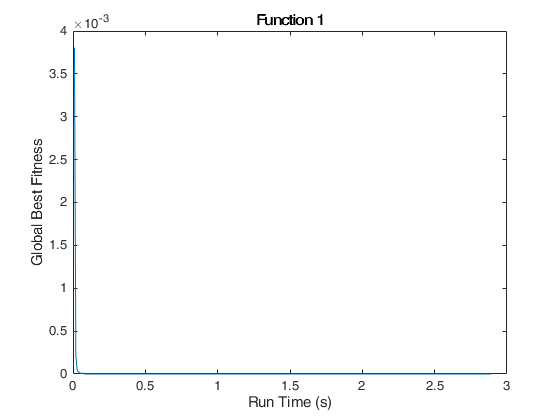
\includegraphics[width=\textwidth]{img/summary/function1}
    \caption{Function 1}
  \end{subfigure}
  \begin{subfigure}[b]{0.4\textwidth}
    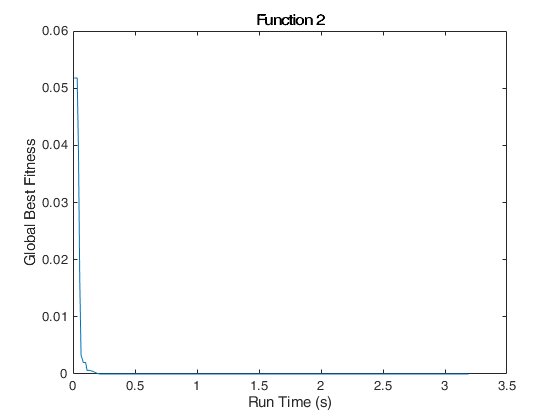
\includegraphics[width=\textwidth]{img/summary/function2}
    \caption{Function 2}
  \end{subfigure}
  \caption{Run-Time vs Best Fitness Achieved of each function}
\end{figure}
\end{frame}

\begin{frame}{Results}
\begin{figure}
  \begin{subfigure}[b]{0.4\textwidth}
    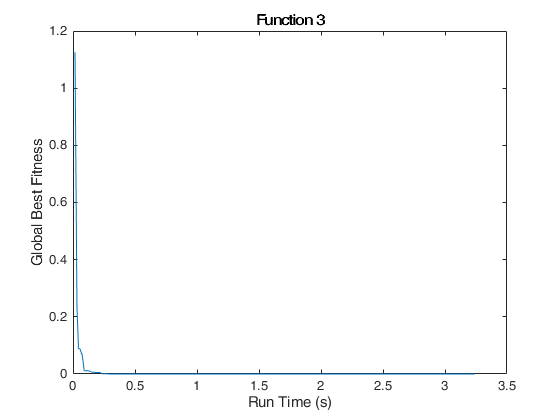
\includegraphics[width=\textwidth]{img/summary/function3}
    \caption{Function 3}
  \end{subfigure}
  \begin{subfigure}[b]{0.4\textwidth}
    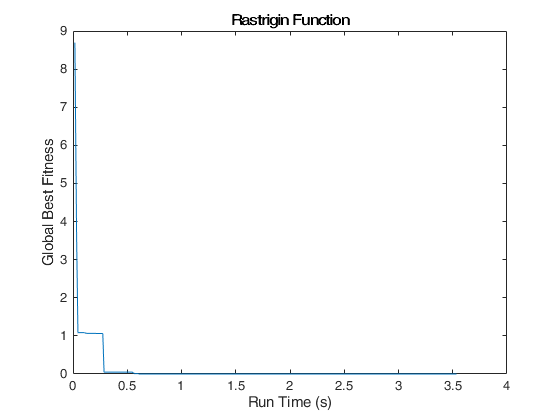
\includegraphics[width=\textwidth]{img/summary/rastrigin}
    \caption{Rastrigin Function}
  \end{subfigure}
  \caption{Run-Time vs Best Fitness Achieved of each function}
\end{figure}
\end{frame}

\begin{frame}{Results}
\begin{figure}
  \begin{subfigure}[b]{0.4\textwidth}
    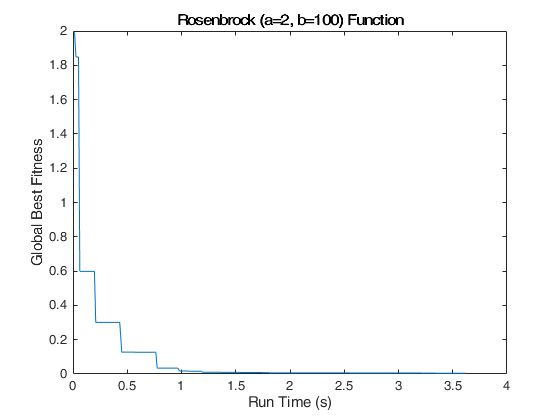
\includegraphics[width=\textwidth]{img/summary/rosenbrock2-100}
    \caption{Rosenbrock (a=2, b=100) Function}
  \end{subfigure}
  \begin{subfigure}[b]{0.4\textwidth}
    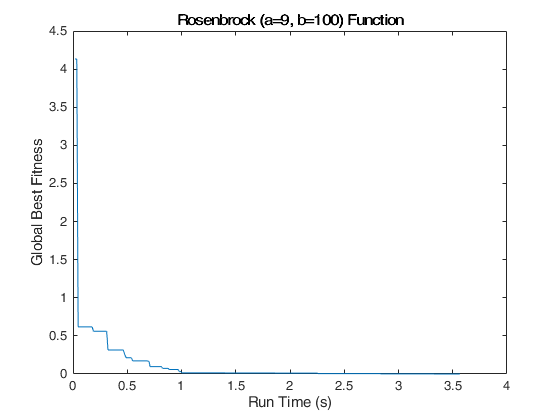
\includegraphics[width=\textwidth]{img/summary/rosenbrock9-100}
    \caption{Rosenbrock (a=9, b=100) Function}
  \end{subfigure}
  \caption{Run-Time vs Best Fitness Achieved of each function}
\end{figure}
\end{frame}

\begin{frame}{CEC 2014 Benchmarks}

CEC is a committee known for creating competitions for optimization algorithms. Each year CEC provides a set of functions that are known for testing optimization algorithms for scientists to submit their work and compare the effectiveness of their algorithms. Each test suite includes functions that are shifted and rotated which are to be run in black box tests though their code is reviewable and written in C++.

The following parameters are set and used in the algorithm.

\begin{align*}
\text{Number of Prides} &= 4\\
\text{Percent of Nomad Lions} &= 0.2\\
\text{Roaming Percent} &= 0.2\\
\text{Mutate Probability} &= 0.2\\
\text{Sex Rate} &= 0.8\\
\text{Mating Probability} &= 0.3\\
\text{Immigrate Rate} &= 0.4\\
\end{align*}
\end{frame}



\begin{frame}{CEC 2014 Benchmarks}
\begin{table}[]
\begin{tabular}{llll}
  \textbf{Type}
    & \textbf{ID} & \textbf{Function} & \textbf{f*} \\ \hline
  Unimodal
    & f1 & Rotated high conditioned elliptic function & 100 \\
    & f2 & Rotated bent cigar function & 200 \\
    & f3 & Rotated discus function & 300 \\
  Multimodal
    & f4 & Shifted and rotated Rosenbrock function & 400 \\
    & f5 & Shifted and rotated Ackley's function & 500 \\
    & f6 & Shifted and rotated Weierstrass function & 600 \\
    & f7 & Shifted and rotated Griewank's function & 700 \\
    & f8 & Shifted Rastrigin function & 800 \\
    & f9 & Shifted and rotated Rastrigin's function & 900 \\
    & f10 & Shifted Schwefel function & 1000 \\
    & f11 & Shifted and rotated Schwefel's function & 1100 \\
    & f12 & Shifted and rotated Katsuura function & 1200 \\
    & f13 & Shifted and rotated HappyCat function & 1300 \\
    & f14 & Shifted and rotated HGBat function & 1400 \\
    & f15 & Shifted and rotated Expanded Griewank's plus Rosenbrock's function & 1500 \\
    & f16 & Shifted and rotated Expanded Scaffer's F6 function & 1600 \\
  Hybrid
    & f17 & Hybrid function1 (f 9, f 8, f 1) & 1700 \\
    & f18 & Hybrid function2 (f 2, f 12, f 8) & 1800 \\
    & f19 & Hybrid function3 (f 7, f 6, f 4, f 14) & 1900 \\
    & f20 & Hybrid function4 (f 12, f 3, f 13, f 8) & 2000 \\
    & f21 & Hybrid function5 (f 14, f 12, f 4, f 9, f 1) & 2100 \\
    & f22 & Hybrid function6 (f 10, f 11, f 13, f 9, f 5) & 2200 \\
  Composition
    & f23 & Composition function1 (f 4, f 1, f 2, f 3, f 1) & 2300 \\
    & f24 & Composition function2 (f 10, f 9, f 14) & 2400 \\
    & f25 & Composition function3 (f 11, f 9, f 1) & 2500 \\
    & f26 & Composition function4 (f 11, f 13, f 1, f 6, f 7) & 2600 \\
    & f27 & Composition function5 (f 14, f 9, f 11, f 6, f 1) & 2700 \\
    & f28 & Composition function6 (f 15, f 13, f 11, f 16, f 1) & 2800 \\
    & f29 & Composition function7 (f 17, f 18, f 19) & 2900 \\
    & f30 & Composition function8 (f 20, f 21, f 22) & 3000
\end{tabular}
\caption{Functions defined by CEC 2014 and used for testing}
\end{table}
\end{frame}

\begin{frame}{CEC 2014 Benchmarks}
\begin{table}[]
\begin{tabular}{llll}
  \textbf{Type}
    & \textbf{ID} & \textbf{Function} & \textbf{f*} \\ \hline
  Unimodal
    & f16 & Shifted and rotated Expanded Scaffer's F6 function & 1600 \\
  Hybrid
    & f17 & Hybrid function1 (f 9, f 8, f 1) & 1700 \\
    & f18 & Hybrid function2 (f 2, f 12, f 8) & 1800 \\
    & f19 & Hybrid function3 (f 7, f 6, f 4, f 14) & 1900 \\
    & f20 & Hybrid function4 (f 12, f 3, f 13, f 8) & 2000 \\
    & f21 & Hybrid function5 (f 14, f 12, f 4, f 9, f 1) & 2100 \\
    & f22 & Hybrid function6 (f 10, f 11, f 13, f 9, f 5) & 2200 \\
  Composition
    & f23 & Composition function1 (f 4, f 1, f 2, f 3, f 1) & 2300 \\
    & f24 & Composition function2 (f 10, f 9, f 14) & 2400 \\
    & f25 & Composition function3 (f 11, f 9, f 1) & 2500 \\
    & f26 & Composition function4 (f 11, f 13, f 1, f 6, f 7) & 2600 \\
    & f27 & Composition function5 (f 14, f 9, f 11, f 6, f 1) & 2700 \\
    & f28 & Composition function6 (f 15, f 13, f 11, f 16, f 1) & 2800 \\
    & f29 & Composition function7 (f 17, f 18, f 19) & 2900 \\
    & f30 & Composition function8 (f 20, f 21, f 22) & 3000
\end{tabular}
\caption{Functions defined by CEC 2014 and used for testing}
\end{table}
\end{frame}

\begin{frame}{CEC 2014 Benchmarks Results}
\begin{table}[]
\begin{tabular}{lllll}
    & \textbf{min}       & \textbf{max}       & \textbf{std}       & \textbf{median}    \\ \hline
f1  & 1.647E+07 & 6.730E+07 & 1.053E+07 & 3.844E+07 \\
f2  & 2.645E+05 & 6.888E+06 & 1.386E+06 & 2.092E+06 \\
f3  & 1.034E+04 & 3.092E+04 & 3.979E+03 & 1.670E+04 \\
f4  & 4.738E+02 & 6.284E+02 & 3.272E+01 & 5.611E+02 \\
f5  & 5.208E+02 & 5.210E+02 & 5.124E-02 & 5.210E+02 \\
f6  & 6.195E+02 & 6.296E+02 & 2.167E+00 & 6.254E+02 \\
f7  & 7.005E+02 & 7.011E+02 & 1.218E-01 & 7.009E+02 \\
f8  & 8.547E+02 & 9.298E+02 & 1.350E+01 & 8.845E+02 \\
f9  & 9.658E+02 & 1.028E+03 & 1.518E+01 & 9.971E+02 \\
f10 & 2.586E+03 & 7.135E+03 & 1.273E+03 & 3.864E+03 \\
f11 & 3.717E+03 & 8.245E+03 & 1.148E+03 & 7.470E+03 \\
f12 & 1.202E+03 & 1.203E+03 & 3.312E-01 & 1.203E+03 \\
f13 & 1.300E+03 & 1.301E+03 & 8.465E-02 & 1.300E+03 \\
f14 & 1.400E+03 & 1.400E+03 & 3.087E-02 & 1.400E+03 \\
f15 & 1.514E+03 & 1.549E+03 & 7.715E+00 & 1.525E+03 \\
\end{tabular}
\caption{Results for LOA under CEC 2014 Benchmark}
\end{table}
\end{frame}

\begin{frame}{CEC 2014 Benchmarks Results}
\begin{table}[]
\begin{tabular}{lllll}
    & \textbf{min}       & \textbf{max}       & \textbf{std}       & \textbf{median}    \\ \hline
f16 & 1.611E+03 & 1.613E+03 & 3.086E-01 & 1.612E+03 \\
f17 & 5.180E+05 & 3.363E+06 & 5.823E+05 & 1.612E+06 \\
f18 & 1.991E+03 & 1.350E+04 & 2.131E+03 & 2.910E+03 \\
f19 & 1.911E+03 & 1.923E+03 & 2.082E+00 & 1.919E+03 \\
f20 & 4.630E+03 & 2.635E+04 & 4.406E+03 & 1.484E+04 \\
f21 & 7.908E+04 & 7.593E+05 & 1.624E+05 & 2.698E+05 \\
f22 & 2.473E+03 & 3.134E+03 & 1.545E+02 & 2.782E+03 \\
f23 & 2.620E+03 & 2.633E+03 & 2.678E+00 & 2.624E+03 \\
f24 & 2.618E+03 & 2.632E+03 & 3.211E+00 & 2.627E+03 \\
f25 & 2.700E+03 & 2.709E+03 & 2.528E+00 & 2.707E+03 \\
f26 & 2.700E+03 & 2.701E+03 & 1.122E-01 & 2.700E+03 \\
f27 & 3.117E+03 & 3.739E+03 & 1.630E+02 & 3.536E+03 \\
f28 & 3.255E+03 & 4.404E+03 & 1.954E+02 & 3.296E+03 \\
f29 & 3.125E+03 & 4.300E+03 & 1.531E+02 & 3.131E+03 \\
f30 & 3.813E+03 & 7.945E+04 & 1.646E+04 & 4.796E+03
\end{tabular}
\caption{Results for LOA under CEC 2014 Benchmark}
\end{table}
\end{frame}

\begin{frame}{Conclusion}
To conclude, the Lion Optimization Algorithm uses a Lion-Pride-Outcast behavior for a population to find solutions or what is thought of as a better territory or a safer place for the population to live in. The algorithm combines the effectiveness of swarm optimization in Prides and individual roaming that provides escaping optimas. It also harnesses Genetic Algorithm through mating in prides. The information exchange between Pride and Nomads is key for stuck prides to escape and for previous nomads to improve solutions.
\end{frame}

\end{document}